\documentclass[conference]{IEEEtran}
\IEEEoverridecommandlockouts
\usepackage{cite}
\usepackage{amsmath,amssymb,amsfonts}
\usepackage{algorithmic}
\usepackage{graphicx}
\graphicspath{{img/}}
\usepackage{textcomp}
\usepackage[table]{xcolor}
\usepackage{verbatim}
\usepackage{tabularx}
\def\BibTeX{{\rm B\kern-.05em{\sc i\kern-.025em b}\kern-.08em
    T\kern-.1667em\lower.7ex\hbox{E}\kern-.125emX}}
\begin{document}



\title{
 Cosmic\\Design Report}

\author{\IEEEauthorblockN{Clay Buxton}
\IEEEauthorblockA{\textit{Computer Engineering, Computer Science} \\
\textit{Elizabethtown College}\\
Elizabethtown, PA \\
buxtonc@etown.edu}
\and
\IEEEauthorblockN{Kevin Carman}
\IEEEauthorblockA{\textit{Computer Engineering, Computer Science} \\
\textit{Elizabethtown College}\\
Elizabethtown, PA \\
carmank@etown.edu}

}

\maketitle

\section{Design Methodology}
\subsection{Overview}
Cosmic is a fully emulated, lightweight, and cross-platform 8-bit computer architecture with a RISC-like instruction set designed alongside a rich GUI interface to test, debug, and run the system.

\subsection{Development}
Before any development of Cosmic began, in-depth research was conducted on processors of the time period, like the Z80 and 6502, to build a feature set that would satisfy the goals we wanted to achieve. We documented how other processors implemented various addressing modes and instructions and how other similar projects implemented their solutions in software.

After everything was mapped out and planned, development began simultaneously with the creation of the GUI interface environment and the backbone code of the processor itself. The GUI was developed to allow for easy debugging throughout the design process and for usability of the final project. At first, it was designed to include nothing but a hex editor, a display for the registers, program counter, and stack pointer, and three buttons to cycle the program counter and reset the processor and memory. The backbone code was made up of two files, a header file and a class file. The header file housed the function prototypes, type declarations, registers, program counter, and stack pointer. The class file defined the functions for fetching, decoding, and executing along with the various addressing types we planned to implement. It was set up to allow for easy implementation of instructions as development carried on.

We worked together for a short time putting some finishing touches on the design and implementing a few opcodes, but split up to work more efficiently. Kevin focused on implementing and testing all of the opcodes for the processor while Clay moved on to start writing the assembler.

The Cosmic assembler is close to done, but requires a little more development to work out the kinks. All the opcodes thus far have been implemented and tested except for the recent addition of interrupt handling. In the upcoming weeks we plan to finish the assembler and to implement unit testing for all the opcodes which means we are right on schedule with what we believed we could achieve this semester.

\subsection{Workflow}
\begin{figure}[h!]
	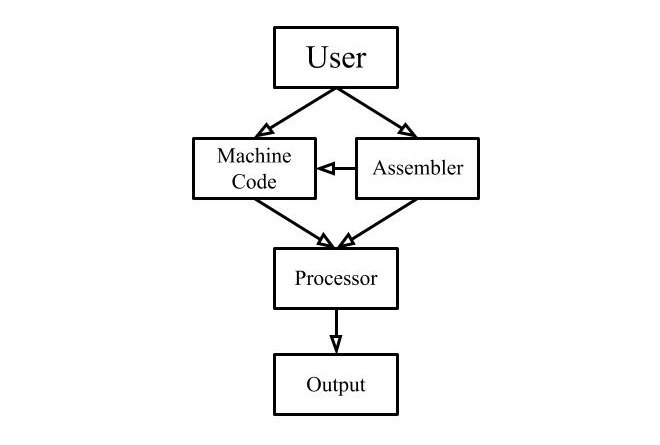
\includegraphics[width=\linewidth]{block_dia.jpg}
	\caption{The Cosmic workflow.}
	\label{fig:The Cosmic Workflow}
\end{figure}

The block diagram in Figure \ref{fig:The Cosmic Workflow} shows the path the user can follow to input their program, run the processor, and obtain the results. Once the user has the GUI up and running, they can input a program written in either assembly or machine code. If the user opts to write their program in assembly, then it will be converted to machine code so that the Cosmic processor can understand it. Currently, the user must manually step the processor to run through their program, but a method to automatically step will be implemented soon. The output of the program is wherever the user specifies it to be, either storing it in memory or leaving it in one of the registers. This is subject to change once we develop the I/O capabilities of Cosmic.

\subsection{Results}


\section{Design Choices}
\subsection{Bitness}
The "bitness" of a chip is traditionally the size of the data bus. An 8-bit chip can address 8 bits of data at one time, a 16-bit chip can address 16 bits of data etc.

Our design choice was between an 8-bit design and a 16-bit design. 32-bit and 64-bit designs were not considered as they did not exist during the time that the chips that Cosmic is similar to were made.\\

\resizebox{\columnwidth}{!}{%
 \begin{tabular}{||c|c|c|c|c||}
 \hline
 Factors & Practical Use & Implementation & Appropriate Design & \cellcolor{blue!40}Total\\ [0.5ex] 
 \hline\hline
 Weights & 3 & 2 & 2& \\ 
 \hline
 8-bit & 5 &  8&  9 & \cellcolor{blue!25}49\\
 \hline
 16-bit  &  8 & 5 &  5 & \cellcolor{blue!25}44\\
 \hline
\end{tabular}
}\\

An 8-bit chip was chosen mainly due to it being more relevant to the class of chips Cosmic is made to fit in with, those of the early 80's and late 70's. A 16-bit chip would have been slightly more work to implement, but would have been much more useful to write for.

\subsection{Registers vs. Zero Page vs In-Memory Registers}

Chips of the time generally had registers in three formats, many registers separated from memory like in the Z80, few registers and then an easily accessible portion of memory like in the 6502, or on chips with onboard memory, the registers would take up the first few bytes of memory.

Each of these has it's pros and cons, but all configurations were designed with two things in mind, speed and utility. On a physical chip, retrieving data from a register is significantly faster than a location in memory, but you only had 8 bytes. Getting something from zero page memory on the 6502 was faster than getting something from another place in memory, but slower than a register, but you had 256 bytes.\\

\resizebox{\columnwidth}{!}{%
 \begin{tabular}{||c|c|c|c|c||}
 \hline
 Factors & Practical Use & Implementation & Appropriate Design & \cellcolor{blue!40}Total\\ [0.5ex] 
 \hline\hline
 Weights & 3 & 2 & 2& \\ 
 \hline
 Many Registers & 9 &  8&  10 & \cellcolor{blue!25}63\\
 \hline
 Zero Page  &  5 & 5 &  10 & \cellcolor{blue!25}45\\
 \hline
 Onboard Memory &  6 & 10 &  7& \cellcolor{blue!25}52\\
 \hline 
\end{tabular}
}\\

Registers, similar to the Z80 made the most sense in our case. Since there is no speed difference between accessing zero page and accessing any other position in memory in our design, zero page addressing would be a waste of time to implement. On-board memory would have been very easy to develop, but was generally found on microcontrollers rather than microprocessors, and would have held no real speed boost either.

\subsection{16-Bit Register Mode}
16-bit register mode is when two of the 8-bit registers can be used together to act as a 16-bit register. This can also be done for certain instructions as well.\\

\resizebox{\columnwidth}{!}{%
 \begin{tabular}{||c|c|c|c|c||}
 \hline
 Factors & Practical Use & Implementation & Appropriate Design & \cellcolor{blue!40}Total\\ [0.5ex] 
 \hline\hline
 Weights & 3 & 2 & 2& \\ 
 \hline
 No 16 Bit mode & 4 &  8&  10 & \cellcolor{blue!25}48\\
 \hline
 16 Bit mode &  10 & 6 &  10 & \cellcolor{blue!25}62\\
 \hline
\end{tabular}
}\\

Overall, a 16-bit mode was a good decision. This allows for a lot more usability, and still fits in with chips of the time since the Z80 also had 16-bit mode instructions. This did add a bit of work, significantly increasing our instruction count,  but was worth it overall.

\subsection{Opcode Selection}

\resizebox{\columnwidth}{!}{%
 \begin{tabular}{||c|c|c|c|c||}
 \hline
 Factors & Practical Use & Implementation & Appropriate Design & \cellcolor{blue!40}Total\\ [0.5ex] 
 \hline\hline
 Weights & 3 & 2 & 2& \\ 
 \hline
 Switch Statement & 0 & 0& 0& \cellcolor{blue!25}48\\
 \hline
 Function Pointers &  0& 0&  0& \cellcolor{blue!25}62\\
 \hline
 Function Pointers with Additional Data &  0 & 0 &  0 & \cellcolor{blue!25}62\\
 \hline
\end{tabular}
}\\

\subsection{Addressing functions}

\resizebox{\columnwidth}{!}{%
 \begin{tabular}{||c|c|c|c|c||}
 \hline
 Factors & Practical Use & Implementation & Appropriate Design & \cellcolor{blue!40}Total\\ [0.5ex] 
 \hline\hline
 Weights & 3 & 2 & 2& \\ 
 \hline
 Individual Functions & 0 &  0&  0 & \cellcolor{blue!25}0\\
 \hline
 Addressing Functions &  0& 0 &  0 & \cellcolor{blue!25}0\\
 \hline
\end{tabular}
}\\

\subsection{GUI Backend}

\resizebox{\columnwidth}{!}{%
 \begin{tabular}{||c|c|c|c|c||}
 \hline
 Factors & Practical Use & Implementation & Appropriate Design & \cellcolor{blue!40}Total\\ [0.5ex] 
 \hline\hline
 Weights & 3 & 2 & 2& \\ 
 \hline
 ImGui & 0 &  0&  0 & \cellcolor{blue!25}0\\
 \hline
 Qt4 &  0 & 0 &  0 & \cellcolor{blue!25}0\\
 \hline
\end{tabular}
}\\


\subsection{Signed vs. Unsigned Data}

\resizebox{\columnwidth}{!}{%
 \begin{tabular}{||c|c|c|c|c||}
 \hline
 Factors & Practical Use & Implementation & Appropriate Design & \cellcolor{blue!40}Total\\ [0.5ex] 
 \hline\hline
 Weights & 3 & 2 & 2& \\ 
 \hline
 Specifically Signed Data & 0 &  0 &  0 & \cellcolor{blue!25}0\\
 \hline
 Overflow and Carry flags &  0 & 0 &  0 & \cellcolor{blue!25}0\\
 \hline
\end{tabular}
}\\

\subsection{Supported Systems}

\resizebox{\columnwidth}{!}{%
 \begin{tabular}{||c|c|c|c|c||}
 \hline
 Factors & Practical Use & Implementation & Appropriate Design & \cellcolor{blue!40}Total\\ [0.5ex] 
 \hline\hline
 Weights & 3 & 2 & 2& \\ 
 \hline
 Windows, macOS, \& Linux & 0 &  0 &  0 & \cellcolor{blue!25}0\\
 \hline
 macOS \& Linux &  0 & 0 &  0 & \cellcolor{blue!25}0\\
 \hline
\end{tabular}
}\\







\end{document}